\section{Semantics}

\begin{frame}{Semantics}
\framesubtitle{Type Checking}

\begin{itemize}
  \item Lack of Type checking in semantics
  \item Matrices and Vectors
\end{itemize}

\begin{equation}
\small
\frac { { e }_{ v },st\vdash { a }_{ 1 }{ \rightarrow  }_{ A }{ v }_{ 1 }\quad { e }_{ v },st\vdash { a }_{ 2 }{ \rightarrow  }_{ A }{ v }_{ 2 } }{ { e }_{ v },st\vdash { a }_{ 1 }+{ a }_{ 2 }{ \rightarrow  }_{ A }{ v } } ,\begin{matrix} v={ v }_{ 1 }+{ v }_{ 2 }, \\ Typeof({ a }_{ 1 }) = Typeof({ a }_{ 2 }) \end{matrix}
\end{equation}

\begin{equation}
\resizebox{.9\textwidth}{!}{

\small
    $\frac { { e }_{ v },st\vdash j{ \rightarrow  }_{ A }{ v }_{ 1 },\quad { e }_{ v },st\vdash k{ \rightarrow  }_{ A }{ v }_{ 2 } }{ { M }^{ 1 }\quad =\quad matrix<mtype>[{ v }_{ 1 },{ v }_{ 2 }]\rightarrow { st }^{ ` },{ e }_{ v } }  ,{ M }^{ 1 }[{ v }_{ 1 },{ v }_{ 2 }]= \begin{bmatrix} { { 0 }_{ 1,1 } } & 0_{ 1,2 } & \dots  & { 0 }_{ { 1,{ v }_{ 2 } } } \\ 0_{ 2,1 } & 0_{ 2,2 } & \dots  & 0_{ 2,v_{ 2 } } \\ \vdots  & \vdots  & \ddots  & \vdots  \\ { 0 }_{ { v }_{ 1 },1 } & 0_{ v_{ 1 },2 } & \dots  & { 0 }_{ { v }_{ 1 },{ v }_{ 2 } } \end{bmatrix}$
    }
\end{equation}

\end{frame}

\begin{frame}{Booleans}
\framesubtitle{Booleans allowed in boolean expression}
\begin{equation}
	\frac { { e }_{ v },st\vdash { a }_{ 1 }{ \rightarrow  }_{ A }{ v }_{ 1 }\quad { e }_{ v },st\vdash { a }_{ 2 }{ \rightarrow  }_{ A }{ v }_{ 2 } }{ { e }_{ v },st\vdash { a }_{ 1 }=={ a }_{ 2 }{ \rightarrow  }true } ,{ v }_{ 1 }={ v }_{ 2 }
\end{equation}

\begin{equation}
	\frac { { e }_{ v },st\vdash { b }_{ 1 }{ \rightarrow  }_{ B }{ B }_{  }\quad { e }_{ v },st\vdash { b }_{ 2 }{ \rightarrow  }_{ B }{ B }_{  } }{ { e }_{ v },st\vdash { b }_{ 1 }=={ b }_{ 2 }{ \rightarrow  }true } 
\end{equation}

\begin{equation}
	\frac { { e }_{ v },st\vdash { b }_{ 1 }{ \rightarrow  }_{ B }{ B }_{ 1 }\quad { e }_{ v },st\vdash { b }_{ 2 }{ \rightarrow  }_{ B }{ B }_{ 2 } }{ { e }_{ v },st\vdash { b }_{ 1 }=={ b }_{ 2 }{ \rightarrow  }false } , { B }_{ 1 } \neq { B }_{ 2 } 
\end{equation}
\end{frame}

\section{Compiler}

    \subsection{Compiler vs. Intrepreter}
    \begin{frame}[t]{Compiler}\framesubtitle{Compiler vs. Intrepreter}
        \begin{itemize}
            \item Performance
            \item Development Cycle
            \item Debugging
            \item Specific Constraints
        \end{itemize}
    \end{frame}

    \subsection{Compiler Overview}
    \begin{frame}[t]{Compiler}\framesubtitle{Compiler Overview}
        \begin{columns}[t]
            \begin{column}{.48\textwidth}
                \begin{itemize}
                    \item ANTLRv4
                    \item Visitor Pattern
                    \item JAVA
                \end{itemize}
        \begin{figure}[ht]
        \centering
        \resizebox{.9\textwidth}{!}{
        \begin{tikzpicture}
            \matrix (m) [ampersand replacement=\&,matrix of nodes]
            {
             GAMBL  \& $\to$ \&  OpenCL C  \\
                \&  Java    \& OpenCL C \& $\to$ \& \hspace{1 em} M \hspace{2 em}  \\
                \&       \&   \& C  \&         \\
                \&       \&               \\
              };
            \draw (m-1-1.south west) |- (m-1-3.north east) |- (m-2-2.north east) |- (m-2-2.south west) |- (m-1-1.south west);
            \draw (m-2-2.south east) |- (m-2-5.north east) --(m-2-5.south east) -- (m-2-5.south west) |- (m-3-4.south west) |- (m-2-2.south east);
        \end{tikzpicture}
        }
        \end{figure}

            \end{column}
            \begin{column}{.48\textwidth}
                \vspace{-30pt}
                \begin{figure}
                    \centering
                    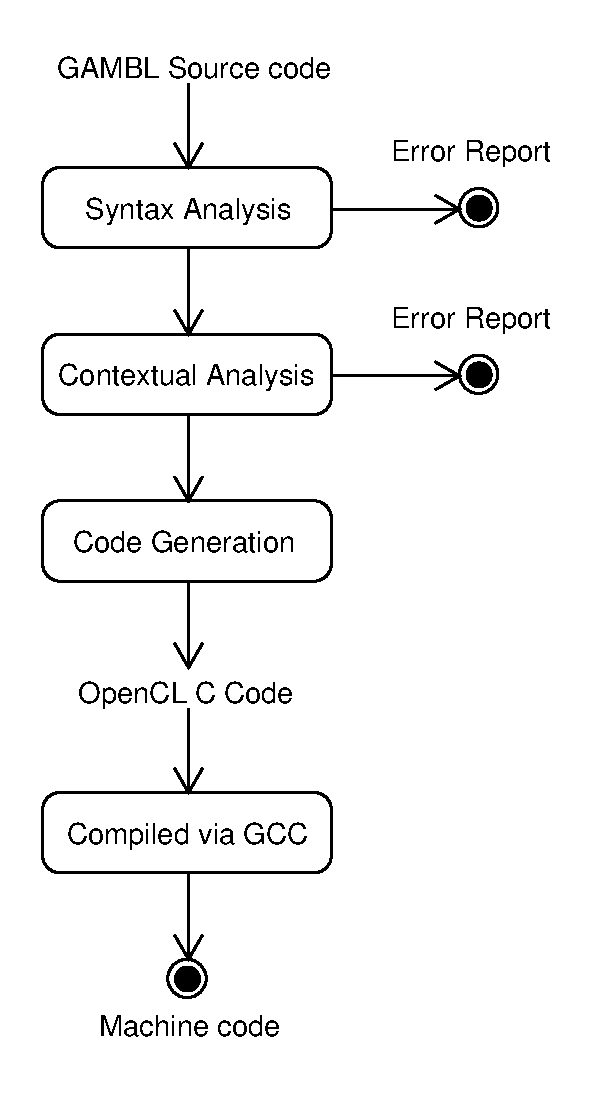
\includegraphics[width=0.8\textwidth]{images/CompilerDiagram.pdf}
                \end{figure}
            \end{column}
        \end{columns}
    \end{frame}